\chapter{Sistemi Informativi e Privacy}

\section{Sistemi Informativi}

\qs{}{Che cos'è un sistema informativo?}

\dfn{Sistema Informativo}{
  Un sistema informativo è un sistema formale, sociotecnico e orgazzativo per collezionare, processare, raccogliere e distribuire informazioni usate da organizzazioni.
}

\cor{Sistema Informativo Computazionale}{
  Un sistema informativo computazionale è un sistema composto da persone e computer ce processano o interpretano informazioni.
}

\paragraph{Lo scopo di un sistema informativo è quello di supportare:}

\begin{itemize}
  \item Le attività (automazione). 
  \item Le decisioni prese dagli alti ranghi di organizzazioni (analisi, controllo, coordinazione, statistica).
\end{itemize}

\paragraph{I sistemi informativi funzionano grazie agli scambi di dati e informazioni:}

\begin{itemize}
  \item Dati modellati come insiemi di processi interconnessi dove l'output di un processo è l'input di un altro processo. 
  \item I dati appartengono a diverse entità: 
    \begin{itemize}
      \item Impiegati. 
      \item Clienti.
      \item Fornitori.
    \end{itemize}
  \item Differenti tipi di dati:
    \begin{itemize}
      \item Identificativi personali. 
      \item Emails.
      \item Dati di processi, transazioni, etc.
    \end{itemize}
\end{itemize}

\paragraph{Un sistema informativo, per essere conforme al GDPR, deve assicurare:}

\begin{itemize}
  \item \fancyglitter{Autorizzazione basata su attributi:} meccanismi per accedere a tutti i dati, sotto determinate circostanze.
  \item \fancyglitter{Anonimizzazione} e \fancyglitter{Pseudoanonimizzazione} dei dati: meccanismi per garantire l'anonimato o lo pseudoanonimato.
  \item \fancyglitter{Tracciabilità:} un registro di chi ha creato, modificato o cancellato informazioni, quando e per quale scopo. 
  \item \fancyglitter{Cancellazione dei dati:} meccanismi per il diritto all'oblio.
\end{itemize}

\subsection{Tecniche di Controllo degli Accessi}

\dfn{Controllo degli Accessi}{
  Si restringe l'accesso alle risorse computazionali, specialmente in sistemi multi-utente.
}

\nt{I requisiti di privacy e sicurezza devono essere mantenuti nel sistema in modo efficiente. Tuttavia in situazioni di emergenza si possono fare delle eccezioni (e.g. in un ospedale con un paziente in pericolo di vita).}

\cor{Role Based Access Control (RBAC)}{
  Formalizzato da NIST nel 1992. Si gestisce l'accesso in base al ruolo invece che a un identificatore. Il ruolo fornisce un livello di astrazione (come collezione di permessi). Ogni ruolo può essere assegnato a un numero arbitrario di utenti.
}

\qs{}{Come funziona RBAC (fig: \ref{fig:rbac})?}

\begin{itemize}
  \item Gli \fancyglitter{amministratori} assegnano permessi a ogni ruolo. 
  \item I ruoli possono essere assegnati a utenti individuali (e ogni utente può avere più ruoli). 
  \item Gli amministratori possono aggiornare i ruoli aggiungendoli o rimuovendoli da determinati utenti.
\end{itemize}

\begin{figure}[h]
    \centering
    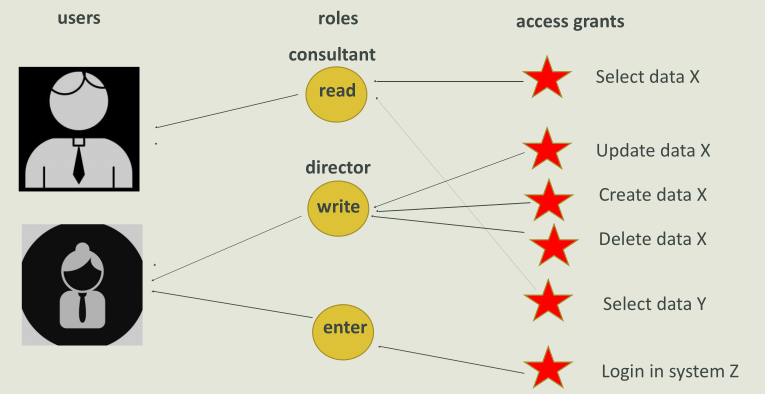
\includegraphics[scale=0.5]{02P/RBAC.png}
    \caption{RBAC.}
    \label{fig:rbac}

  \end{figure}

\paragraph{Limiti di RBAC:}

\begin{itemize}
  \item Non fornisce un meccanismo flessibili per cui i clienti possano esprimere dei loro requisiti. 
  \item Non cattura lo scopo per cui i dati vengono rilasciati. 
  \item Per cui RBAC si evolve in Attribute Base Access Control (ABAC).
\end{itemize}

\paragraph{Aggiungendo contesto, le decisioni autorizzative possono essere basate su:}

\begin{itemize}
  \item Ruolo. 
  \item Persone od oggetti collegati all'utente. 
  \item Di che cosa si ha bisogno. 
  \item Dove l'utente vuole accedere. 
  \item Quando l'utente vuole accedere. 
  \item Com'è l'utente vuole accedere a quelle informazioni.
\end{itemize}

\cor{Attribute Based Access Control (ABAC)}{
  Definendo un contesto si possono aggiungere adeguate politiche di accesso che definiscono in maniera dichiarativa come debba avvenire l'accesso.
}

\nt{Conoscere il ruolo di un utente non è abbastanza per assicurare la sicurezza. Si richiede il contesto e le relazioni tra le varie entità presenti nel sistema.}

\paragraph{Caratteristiche di ABAC(fig: \ref{fig:abac}):}

\begin{itemize}
  \item Adotta un approccio \fancyglitter{policy driven}. 
  \item Usa gli attributi \fancyglitter{soggetto}, \fancyglitter{oggetto} e \fancyglitter{ambiente}. 
  \item Rimuove la necessità di dover essere registrati in un sistema per essere in grado di accedere a risorse condivise.
  \item Utilizza un \fancyglitter{authorization engine} (fig: \ref{fig:auth}).
\end{itemize}

\begin{figure}[h]
    \centering
    \begin{minipage}{0.45\textwidth}
        \centering
        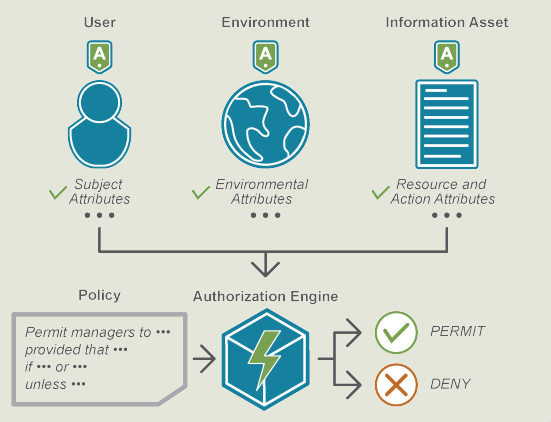
\includegraphics[width=\linewidth]{02P/ABAC.png}
        \caption{ABAC.}
        \label{fig:abac}
    \end{minipage}
    \hfill
    \begin{minipage}{0.45\textwidth}
        \centering
        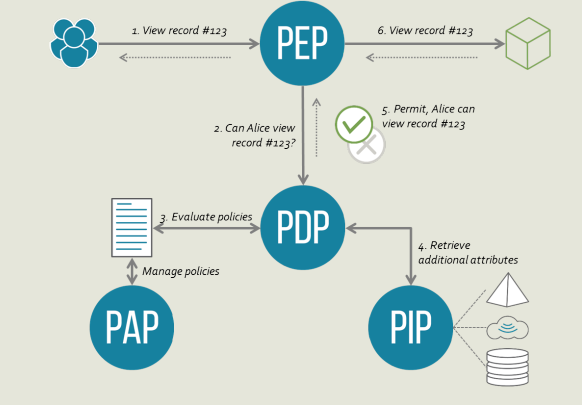
\includegraphics[width=\linewidth]{02P/engine.png}
        \caption{Dettaglio dell'authorization engine.}
        \label{fig:auth}
    \end{minipage}
\end{figure}

\nt{Le policies sono espresse in XACML (eXtensible Access Control Markup Language).}

\section{Pseudoanonimizzazione con Crittografia}

\dfn{Pseudoanonimizzazione}{
  La pseudoanonimizzazione è una procedura di data management e di deidentificazione per cui informazioni identificabili in un record sono rimpiazzate da uno o più identificatori artificiali (pseudonimi).
}

\nt{Un singolo pseudonimo viene utilizzato in modo consistente per permettere un'analisi accurata. Tuttavia questi dati pseudoanonimizzati possono essere riportati al loro stato originale perché viene salvata l'associazione con lo pseudonimo.}

\cor{Crittografia su Colonne}{
  La Crittografia su colonne è una feature per proteggere dati sensibili nei databases. Permette di crittografare dati sensibili senza rivelare la chiave all'engine del database. Questo fornisce una separazione tra:

  \begin{itemize}
    \item Chi possiede i dati e può visualizzarli. 
    \item Chi gestisce i dati, ma non ha il diritto di accedervi.
  \end{itemize}
}

\paragraph{Ci sono due tipi di chiavi:}

\begin{itemize}
  \item \fancyglitter{Column encryption keys:} per crittografare il dato. 
  \item \fancyglitter{Column master keys:} per crittografare la column encryption key.
\end{itemize}

\nt{Le chiavi non sono mai memorizzate nei meta dati, ma vengono salvate in un repository esterno.}

\paragraph{Crittografia deterministica vs. randomizzata:}

\begin{itemize}
  \item \fancyglitter{Crittografia deterministica:} genera sempre gli stessi valori per ogni testo. 
  \item \fancyglitter{Crittografia randomizzata:} utilizza valori casuali. È più sicura, ma impedisce le ricerche sul database.
    
\end{itemize}

\paragraph{Rivest-Shamir-Adleman (RSA):}

\begin{itemize}
  \item È un sistema crittografico a chiave pubblica. 
  \item Gli utenti creano e pubblicano una chiave pubblica basata su due numeri primi sufficientemente grandi segreti.
  \item I messaggi possono essere crittati da chiunque usando la chiave pubblica. 
  \item Possono essere decrittati solo da chi conosce la chiave privata.
  \item Utilizza anche un sistema di padding.
\end{itemize}

\paragraph{TDE (Oracle):}

\begin{itemize}
  \item Si usa sempre una sola chiave di crittografia. 
  \item Nessuna chiave è salvata in chiaro. 
  \item Il repository esterno di Oracle è chiamato Oracle wallet. 
  \item Vengono separate le responsabilità per prevenire accessi illeciti.
\end{itemize}

\subsection{Tracciabilità mediante Auditing}

\dfn{Auditing}{
  L'auditing è il processo di esaminazione e validazione di documenti, dati, processi, procedure, sistemi.
}

\cor{Audit Log}{
  Documento in cui si memorizzano in ordine cronologico tutte le attività di interesse.
}

\cor{Audit Objectives}{
  Insieme di business rules, controlli di sistema, regolazioni di governi, policies di sicurezza.
}

\paragraph{Altre definizioni:}

\begin{itemize}
  \item \fancyglitter{Auditor:} persona autolizzata a fare audit. 
  \item \fancyglitter{Audit procedure:} insieme di istruzioni per il processo di auditing. 
  \item \fancyglitter{Audit report:} documento contenente tutti i risultati dell'audit.
  \item \fancyglitter{Audit trail:} record cronologico di cambiamenti su documenti e dati, attività di sistema od operazioni.
\end{itemize}

\paragraph{Tipi di audit:}

\begin{itemize}
  \item Interno: esaminazione di attività condotte da membri dello staff. 
  \item Esterno: esaminazione di attività condotte da terze parti.
\end{itemize}

\paragraph{Attività di auditing (fig: \ref{fig:auditing}):}

\begin{itemize}
  \item Identificare problemi di sicurezza. 
  \item Stabilire piani, politiche e procedure. 
  \item Assicurarsi che gli elementi contrattuali siano riscontrati. 
  \item Organizzare incontri tra team di verifica. 
\end{itemize}

\begin{figure}[h]
    \centering
    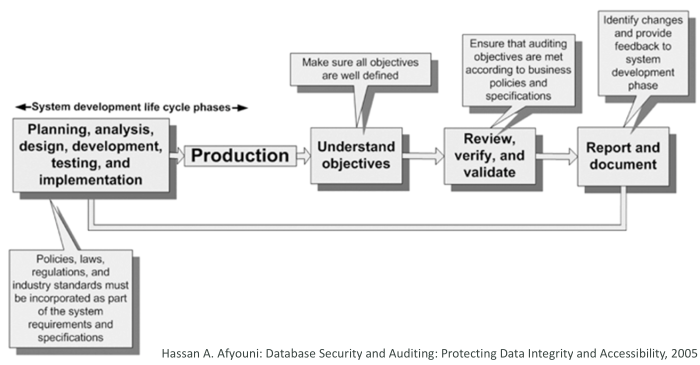
\includegraphics[scale=0.53]{02P/auditing.png}
    \caption{Processo di auditing.}
    \label{fig:auditing}

  \end{figure}

\paragraph{Modelli di auditing:}

\begin{itemize}
  \item \fancyglitter{Modello 1:}
    \begin{itemize}
      \item Registra le entità in un repository. 
      \item Tiene traccia delle attività performate.
    \end{itemize}
  \item \fancyglitter{Modello 2:}
    \begin{itemize}
      \item Memorizza solo i valori delle colonne. 
      \item C'è un meccanismo di archiviazione. 
      \item Non registra le azioni performate sui dati. 
      \item Ideale per fare auditing di una o due colonne di una tabella.
    \end{itemize}
\end{itemize}

\section{Controllo del Rilascio di Informazioni Statistiche}

\paragraph{I databases sono risultati del collezionamento di dati di diversa provenienza:}

\begin{itemize}
  \item Web. 
  \item Social media. 
  \item Smartphones. 
  \item etc.
\end{itemize}

\nt{Molte di queste informazioni sensibili potrebbero essere utili per un'analisi dei dati.}

\paragraph{Spesso i dati per scopi statistici sono rilasciati come:}

\begin{itemize}
  \item Open data: uso del web per rappresentare i legami tra le pagine. 
  \item Datasets per riproducibilità degli esperimenti. 
  \item Data challenge. 
  \item Politiche/Regolamenti.
\end{itemize}

\nt{In alcuni casi (e.g. Netflix nel 2006) i dati sono stati usati per inferire informazioni oltre lo scopo per cui sono stati rilasciati.}

\subsection{Disclosure}

\dfn{Disclosure}{
  Un disclosure può:
  \begin{itemize}
    \item Occorrere basandosi solamente sui dati rilasciati. 
    \item Risultare da combinazioni dei dati rilasciati con dati esterni che potrebbero o meno essere disponibili al pubblico.
  \end{itemize}
}

\paragraph{Macrodata e Microdata:}

\begin{itemize}
  \item \fancyglitter{Macrodata:} spesso ottenuta con aggregazioni di tipo statistico:
    \begin{itemize}
      \item \evidence{Conti/Frequenza:} ogni cella di una tabella contiene il conto o la frequenza delle situazioni.
      \item \evidence{Magnitudo:} ogni cella di una tabella contiene un valore aggregato di una quantità di interesse.
    \end{itemize}
  \item \fancyglitter{Microdata:} grana fine, su singole persone (rischio maggiore di data breach).
\end{itemize}

\qs{}{Come può avvenire questo rilascio non voluto di informazioni?}

\begin{itemize}
  \item Inferenza su sondaggi statistici (inferential disclosure):
    \begin{itemize}
      \item Avviene quando le informazioni possono essere inferite con alta confidenza per via di proprietà statistiche dei dati. 
      \item Questo tipo di disclosure è difficilmente gestibile perché in linea teorica si può fare inferenza su qualsiasi dato e quindi nessun dato potrebbe essere rilasciato. 
      \item L'inferenza serve per predirre aggregati, non singoli valori.
    \end{itemize}
  \item Informazioni sensibili (attribute disclosure):
    \begin{itemize}
      \item Avviene se si riescono a stimare le informazioni di un attributo.
    \end{itemize}
  \item Direttamente sui dati rilasciati (identity disclosure):
    \begin{itemize}
      \item Avviene quando una terza parte può identificare il soggetto. 
      \item Nel caso dei macrodata non è particolarmente pericoloso. 
      \item Per i microdata è un problema perché sono più personali.
    \end{itemize}
\end{itemize}

\nt{I microdata contengono specifici identificatori: nome, numero telefonico, email, codice fiscale, etc. Il primo step per trattare i microdata è quello di eliminare o crittografare quelle colonne.}

\subsection{Statistical Disclosure Control}

\dfn{Statistical Disclosure Control}{
  È una collezione di metodi che sono usati come parte del processo di anonimizzazione per controllare l'accesso ai dati.
}

\nt{Quest'attività non è strettamente considerata a favore della privacy (fig: \ref{fig:data}).}

\begin{figure}[h]
    \centering
    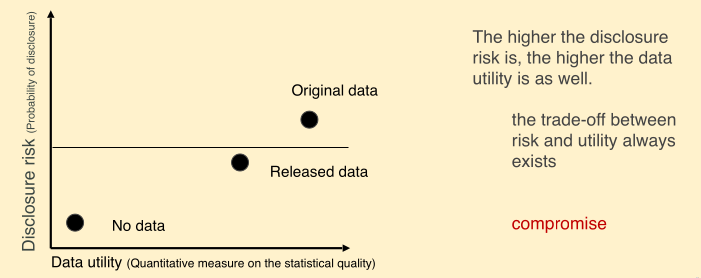
\includegraphics[scale=0.6]{02P/data.png}
    \caption{Utilità vs. Privacy.}
    \label{fig:data}

\end{figure}

\begin{figure}[h]
    \centering
    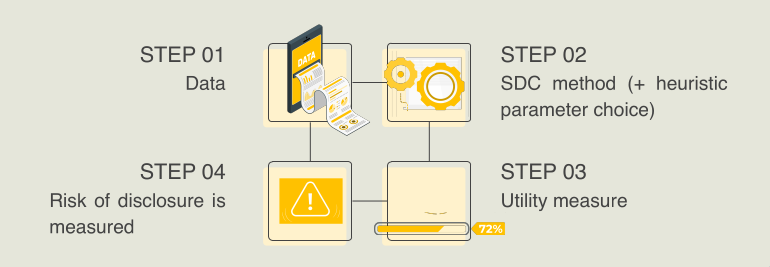
\includegraphics[scale=0.65]{02P/SDC.png}
    \caption{Ciclo di Statistical Disclosure Control (SDC).}
\end{figure}

\paragraph{I passi per proteggere i dati sono:}

\begin{enumerate}
  \item Definire i \fancyglitter{quasi identificatori}. 
  \item Una piccola percentuale di quasi identificatori (generalmente meno del 5\%) possono essere identificati.
  \item Calcolare le frequenze per le combinazioni di quasi identificatori. 
  \item Effettuare il \fancyglitter{recoding} dei valori degli attributi (e.g. discretizzazione\footnote{Associare un valore costante di un intervallo associato a un valore continuo.}). 
  \item Applicare metodi SDC. 
  \item Effettuare una soppressione locale delle variabili di identificazione se ci sono ancora dei records che richiedono protezione.
\end{enumerate}

\paragraph{Metodi SDC per i macrodata:}

\begin{itemize}
  \item \fancyglitter{Non-perturbativi:} non modificano i valori delle celle:
    \begin{itemize}
      \item Soppressione della cella (CS, Cell Suppression). 
    \end{itemize}
  \item \fancyglitter{Perturbativi:} modificano i valori delle celle: 
    \begin{itemize}
      \item Arrotondamento casuale dei valori nelle celle (RR, Random Rounding). 
      \item Arrotondamento controllato dei valori nelle celle (CR, Controlled Rounding). 
      \item Se con tabelle statistiche si possono modificare le frequenze (CTA, Controlled Tabular Adjustment).
    \end{itemize}
\end{itemize}


\dfn{Cell Suppression}{
  In una tabella si possono sopprimere delle celle (fig: \ref{fig:cs}): 
  \begin{itemize}
    \item Soppressione primaria: non si pubblicano le celle ritenute a rischio. 
    \item Soppressione secondaria: non si pubblicano celle non a rischio per aumentare la protezione delle celle a rischio.
  \end{itemize}
}

\begin{figure}[h]
    \centering
    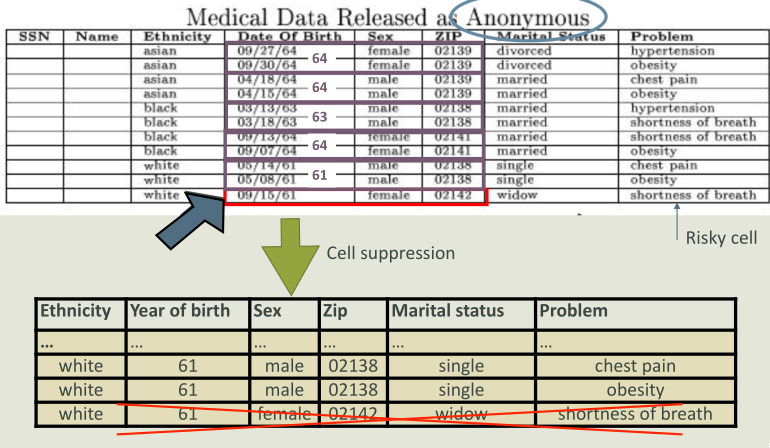
\includegraphics[scale=0.4]{02P/cs.png}
    \caption{Esempio di Cell Suppression.}
    \label{fig:cs}
\end{figure}

\dfn{Rounding e Tabular}{
\begin{itemize}
  \item Random Rounding: viene deciso in modo randomico se effettuare un arrotondamento per difetto o per eccesso.
  \item Controlled Rounding: arrotondamento classico.
  \item Controlled Tabular Adjustment (fig: \ref{fig:rt}): i valori delle celle sensibili sono rimpiazzati da valori simili e le altre celle sono modificate di conseguenza per correggere i valori totali delle righe e delle colonne.
\end{itemize}
}

\begin{figure}[h]
    \centering
    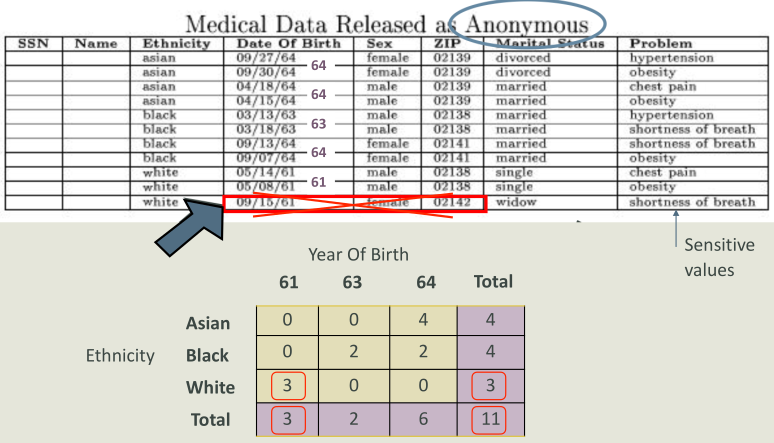
\includegraphics[scale=0.4]{02P/rt.png}
    \caption{Esempio di CTA.}
    \label{fig:rt}
\end{figure}

\paragraph{Metodi SDC per query:}

\begin{itemize}
  \item \fancyglitter{Perturbativi:} si può applicare una perturbazione sia all'input della query che all'output.
  \item \fancyglitter{Restrittivi:} si rifiuta di rispondere a certe query.
\end{itemize}

\paragraph{Metodi SDC per i microdata:}

\begin{itemize}
  \item \fancyglitter{Data Masking:} genera versioni modificate dei microdata.
  \item \fancyglitter{Data Synthesis:} genera versioni sintetiche dei microdata.
\end{itemize}

\begin{figure}[h]
    \centering
    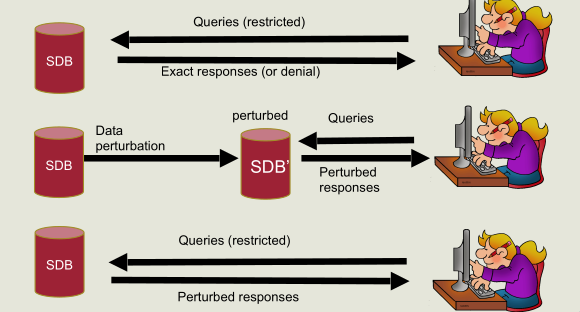
\includegraphics[scale=0.4]{02P/query.png}
    \caption{Sicurezza di databases statistici (SDB).}
\end{figure}

\dfn{Masking Perturbativo}{
  \begin{itemize}
    \item Aggiunta di rumore: 
      \begin{itemize}
        \item Aggiungere a ogni record un rumore. 
        \item Media e correlazioni possono essere preservate. 
      \end{itemize}
    \item Microaggressioni: 
      \begin{itemize}
        \item Partizionare i records in gruppi (basati su similarità). 
        \item Solo la media per ogni gruppo è pubblicata.
      \end{itemize}
    \item Data swapping: 
      \begin{itemize}
        \item I valori per ogni attributo sono ordinati in ordine crescente. 
        \item I valori sono scambiati casualmente in un range ristretto. 
      \end{itemize}
    \item Post randomizzazione:
      \begin{itemize}
        \item Lavora su attributi categorici. 
        \item Gli attributi sensibili sono cambiati secondo determinate matrici.
      \end{itemize}
  \end{itemize}
}

\dfn{Masking non Perturbativo}{
  \begin{itemize}
    \item Sampling: pubblicare un campione dei dati originali. 
    \item Generalizzazione: 
      \begin{itemize}
        \item Gli attributi categorici sono combinati in categorie meno specifiche. 
        \item Gli attributi numerici sono sostituiti da intervalli.
      \end{itemize}
    \item Top/Bottom coding: valori sopra/sotto un threshold sono sostituiti da un estremo (simile all'arrotondamento, ma adattativo). 
    \item Soppressione locale:
      \begin{itemize}
        \item Alcuni attributi sono sostituiti. 
        \item Aumentare la dimensione dei gruppi.
      \end{itemize}
  \end{itemize}
}

\paragraph{Sintesi dei dati per i microdata:}

\begin{itemize}
  \item \fancyglitter{Goal:} rilasciare un dataset mantenendo i dati confidenziali.
  \item \fancyglitter{Metodi:}
    \begin{itemize}
      \item \evidence{Fully Synthetic Data:} sintetizzare tutto il dataset. 
      \item \evidence{Partially Synthetic Data:} sintetizzare solo le variabili sensibili.
    \end{itemize}
  \item \fancyglitter{Problemi:}
    \begin{itemize}
      \item I dati sintetizzati devono avere validità per analisi statistiche.
      \item La sintesi dei dati dipende dal modello usato. 
        \item \evidence{Overfitting:} records sintetici troppo simili ai records originali potrebbero favorire la reidentificazione.
    \end{itemize}
\end{itemize}

\nt{Spesso è difficile misurare l'utilità perché non si sa cosa si voglia fare sui dati. Si potrebbe avere \fancyglitter{perdita di informazioni} (più è grande peggio è).}

\paragraph{Perdita di informazioni per macrodata:}

\begin{itemize}
  \item \fancyglitter{Cell Suppression:} misura del numero delle soppressioni.
  \item \fancyglitter{Rounding and Tabular:} somma delle distanza tra i valori veri e quelli perturbati.
\end{itemize}

\paragraph{Perdita di informazioni per query:}

\begin{itemize}
  \item \fancyglitter{Perturbazione:} differenza tra query non perturbata e query effettiva.
  \item \fancyglitter{Restrizione:} il numero di query rifiutate.
\end{itemize}

\paragraph{Perdita di informazioni per microdata:}

\begin{itemize}
  \item Valutazione di quanto SDC cambi l'output di un'analisi. 
  \item Altre misure base (statistiche, punteggi, distanze, etc.). Si vanno a calcolare le divergenze di Kullback-Leibler (KL) e di Jensen-Shannon (JS).
\end{itemize}

\subsection{Divergenze di Kullback-Leibler e Jensen-Shannon}

\dfn{Kullback-Leibler}{
  La divergenza misura quanto una distribuzione di probabilità perturbata $P(x)$ sia diversa dalla distribuzione di probabilità originaria $Q(x)$ con $x$ il valore di una varibile casuale. È definita come l'entropia relativa di $P$ dato $Q$: 

$$KL(P \parallel Q) = \sum_{x \in \mathcal{X}} P(x) \log \left( \frac{P(x)}{Q(x)} \right)$$

}

\nt{Però KL non è simmetrica, per cui si introduce JS.}

\dfn{Jensen-Shannon}{
 La divergenza misura la similarità mediante KL. Tuttavia JS la simmetrizza ed effettua smoothing: 

$$JS(P \parallel Q) = \frac{1}{2} KL(P \parallel M) + \frac{1}{2} KL(Q \parallel M) \\
\text{with } M = \frac{1}{2}(P + Q)$$

}
